\documentclass{article}
\usepackage[T1]{fontenc}
\usepackage{lmodern}
\usepackage{graphicx}
\usepackage{amsmath,amssymb}
\usepackage[a4paper,margin=2cm]{geometry}
\usepackage[absolute,overlay]{textpos}
\setlength{\TPHorizModule}{1mm}
\setlength{\TPVertModule}{1mm}
\usepackage[indonesian]{babel}
\usepackage{hyperref}
\setlength{\emergencystretch}{2em}
% unit: Halaman 75

\begin{document}

% === Halaman 75 (llm) ===

2. Jika dua huruf terdapat pada kolom kunci yang sama maka tiap huruf diganti dengan huruf di bawahnya (bersifat siklik).

\vspace{10mm}

\vspace{10mm}

Cipherteks: PX \hspace{5cm} Cipherteks: WL

% deskripsi: Ilustrasi kriptografi Playfair untuk kasus bigram 'nq' di mana kedua huruf berada dalam satu kolom, menunjukkan pergeseran huruf ke bawah secara siklik untuk menghasilkan cipherteks PX.
% bbox normalisasi: [0.1200, 0.3000, 0.3400, 0.7500]
\begin{textblock*}{46.20mm}(25.20mm,89.10mm)
\noindent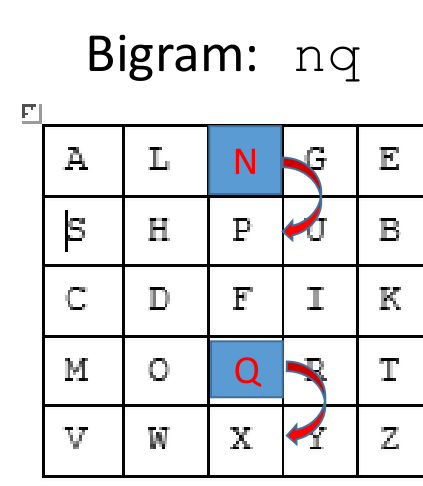
\includegraphics[width=46.20mm,height=133.65mm]{../../images/llm/page_075_img_01.png}%
\end{textblock*}

% deskripsi: Ilustrasi kriptografi Playfair untuk kasus bigram 'ow' di mana kedua huruf berada dalam satu kolom, menunjukkan pergeseran huruf ke bawah secara siklik untuk menghasilkan cipherteks WL.
% bbox normalisasi: [0.6100, 0.3000, 0.8300, 0.7800]
\begin{textblock*}{46.20mm}(128.10mm,89.10mm)
\noindent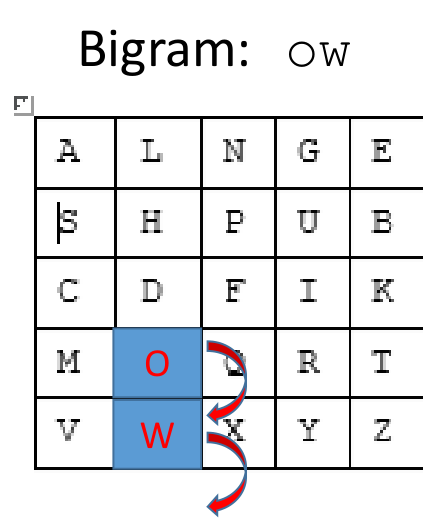
\includegraphics[width=46.20mm,height=142.56mm]{../../images/llm/page_075_img_02.png}%
\end{textblock*}

\end{document}
